\section{Эксперименты}
\subsection*{Экспериментальный пайплайн}
Для исследования принципиальной возможности ускорения подбора гиперпараметров была использована задача классификации изображений на датасете CIFAR-10~\cite{krizhevsky2009learning}.
Нейросеть представляет из себя 2 свёрточных и 2 полносвязных слоя с \verb|MaxPool2d| и активациями \verb|ReLU|.
\begin{figure}[ht]
    \centering
    \includegraphics*[width=\linewidth]{imgs/net.png}
    \caption{Архитектура использованной нейронной сети}
\end{figure}
В качестве целевого лосса стандартно выбрана кросс-энтропия, оптимизация с использованием оптимизатора Adam.
В качестве гиперпараметров были выбраны:
\begin{itemize}
    \item Learning rate
    \item Количество эпох
    \item Label smoothing в кросс-энтропийном лоссе
    \item Weight Decay для Adam
\end{itemize}

Для оптимизации гиперпараметров был использован один из широко распространённых фреймворков Optuna~\cite{optuna_2019}.
Используемый метод --- Tree-structured Parzen Estimator~\cite{bergstra2011algorithms}.
Замечу, однако, что конкретный метод семплирования не имеет значения для данной работы.
Области поиска параметров представлены на таблице~\ref{tab:hyp}.
\begin{table}[ht]
    \begin{tabular}{llll}
    Параметр        & Тип   & Левая граница & Правая граница \\ \hline
    Learning Rate   & float & $10^{-4}$     & $10^{-2}$      \\ \hline
    Weight Decay    & float & $0$           & $10^{-3}$      \\ \hline
    Label Smoothing & float & $0$           & $1$            \\ \hline
    \#epochs        & int   & 5             & 20
    \end{tabular}
    \caption{Области значений гиперпараметров}
    \label{tab:hyp}
\end{table}
Дополнительно для Learning Rate было выбрано лог-равномерное распределение, чтобы точнее отразить влияние этого параметра.
Бюджет для исследования --- 100 обучений.
В ходе каждого эксперимента сеть обучалась с выбранными значениями гиперпараметров и после каждой эпохи значения показателя CKA сохранялись.
Сама оптимизация гиперпараметров происходила при помощи оценки точности на валидационной части датасета.
Показатель CKA при этом считался по выходам двух свёрточных и двух полносвязных слоёв на одном батче валидационной выборки.

Для исследования предлагается простейшая техника отсечения испытания по порогу метрики \textit{CKA}: заранее выбирается порог и если через заданное число $k$ эпох \textit{CKA}
оказывается больше порога, то дальше обучение не продолжается.

\subsection*{Результаты}
На рисунке~\ref{fig:result} приведены графики корреляции \textit{CKA} и итоговой точности на валидационной части датасета в зависимости от числа эпох $k$ перед отсечением.
\begin{figure}[ht]
  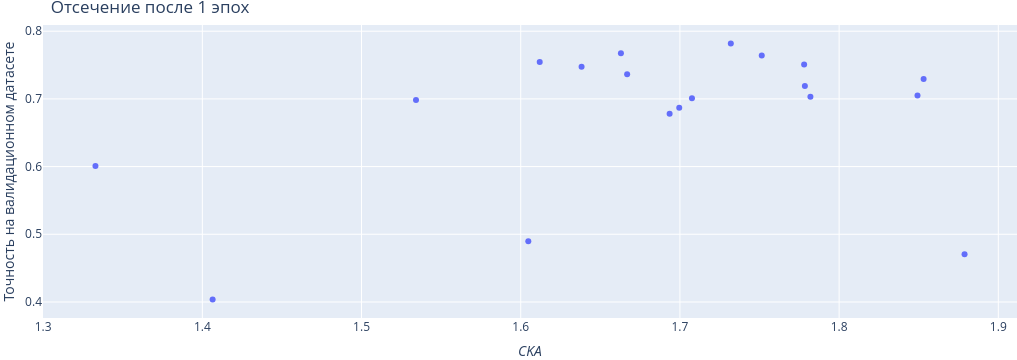
\includegraphics[width=\linewidth]{imgs/1_epochs.png}
  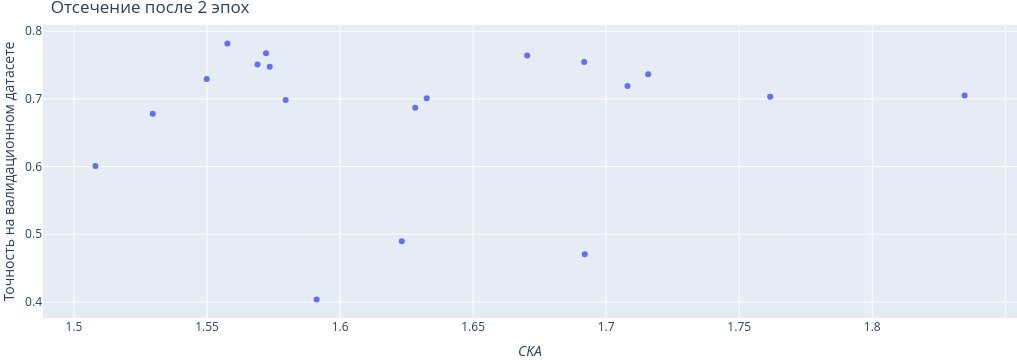
\includegraphics[width=\linewidth]{imgs/2_epochs.png}
  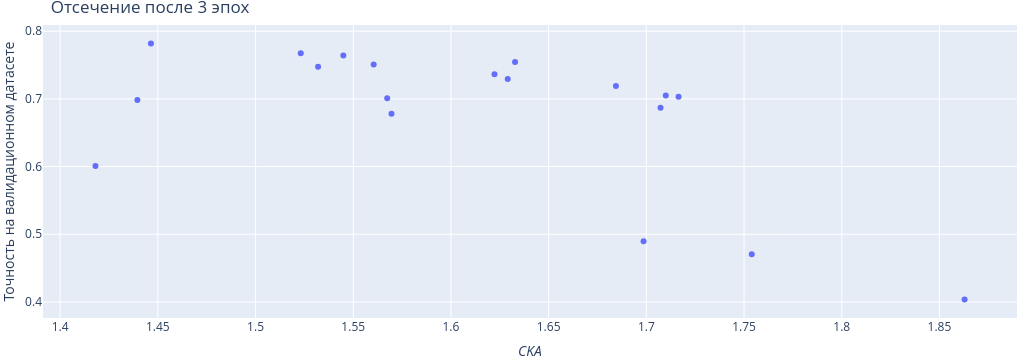
\includegraphics[width=\linewidth]{imgs/3_epochs.png}
  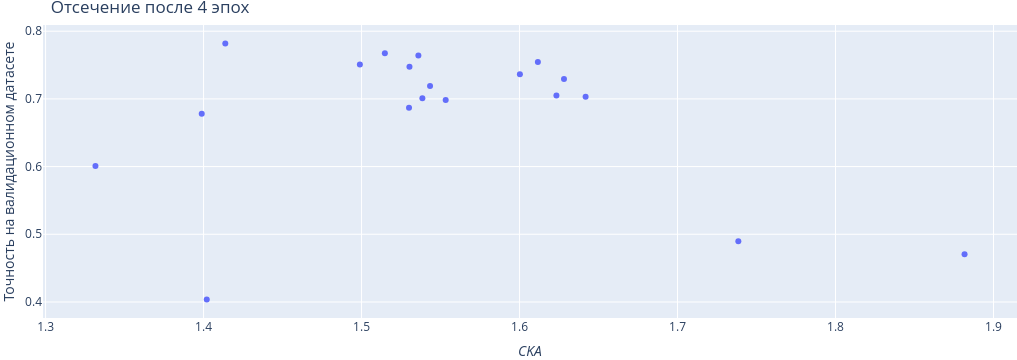
\includegraphics[width=\linewidth]{imgs/4_epochs.png}
  \label{fig:result}
  \caption{Результаты экспериментов}
\end{figure}
Несмотря на то, что подбор гиперпараметров может быть произведён на 100 эпохах, такой эксперимент закончился неудачей из-за технических сложностей, которые не было возможности вовремя устранить.
Тем не менее, он был проведён в сокращённом варианте на 19 испытаниях.

Можно заметить, что после первой эпохи, как и после второй, корреляция практически не просматривается.
Однако уже после третьей, а особенно после четвёртой, корреляция становится всё более чёткой.
Это позволяет выбрать порог, например, в $CKA = 1.5$, при достижении которого обучение можно прерывать.
Данная оптимизация позволит отсечь более 80\% испытаний после 4 эпохи, тем самым значительно сократив время исследования.

Также представляет интерес выбор порога для отсечения обучения после \textit{половины} эпох.
График для этого эксперимента представлен на рисунке
\begin{figure}[ht]
    \centering
    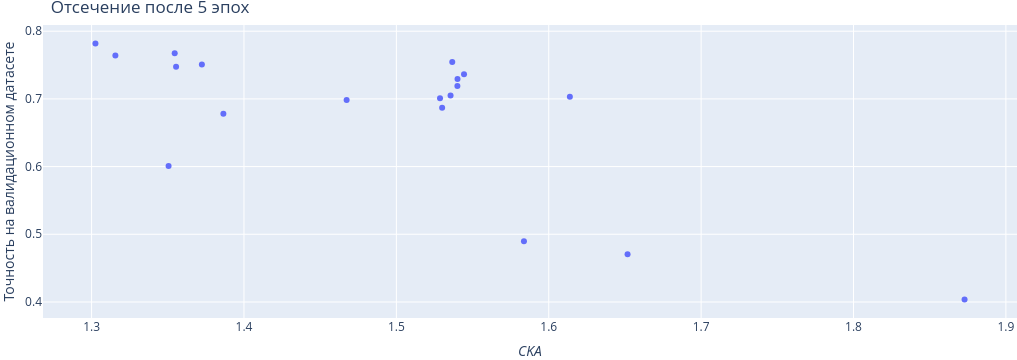
\includegraphics[width=\linewidth]{imgs/half_epochs.png}
    \caption{Отсечение после половины эпох}
\end{figure}
Очевидно, здесь также подходит порог $CKA = 1.5$.
